\documentclass[11pt]{article}

\usepackage[T1]{fontenc}
\usepackage{amsmath,amssymb,amsthm,mathtools}
\usepackage{geometry}
\usepackage{graphicx}
\usepackage{microtype}
\usepackage{enumitem}
\usepackage[hidelinks]{hyperref}
\geometry{margin=1in}

\newtheorem{theorem}{Theorem}
\newtheorem{proposition}{Proposition}
\newtheorem{lemma}{Lemma}
\newtheorem{corollary}{Corollary}
\theoremstyle{remark}
\newtheorem{remark}{Remark}

\newcommand{\T}{\mathbb T}
\newcommand{\R}{\mathbb R}
\newcommand{\C}{\mathbb C}
\newcommand{\Z}{\mathbb Z}
\newcommand{\eps}{\varepsilon}
\newcommand{\cO}{\mathcal O}
\newcommand{\ee}{\mathrm e}

\title{Two sharp obstructions to the Boutet de Monvel conjecture:\\
curvature, reversibility, and a flat-torus characterization}
\author{Candidate counterexamples for arXiv:2110.09389\\
Run \texttt{fa\_banach\_001}, lane 10, model GPT5.6}
\date{22 July 2026}

\begin{document}
\maketitle

\begin{center}
\fbox{\parbox{0.92\linewidth}{
\textbf{Status.} Candidate counterexample likely valid, independently of the
meaning assigned to ``strictly convex.''  The strongly convex multiplier
$P=(-\Delta)^{1/2}+cD_1$ on $\T^n$ satisfies every printed hypothesis of
Winterrose's Conjecture~4.1, including everywhere positive curvature of its
unit co-ball, but conclusion~(4) fails.  A second example,
$P=\partial_1^4+\partial_2^4$, shows that segment-strict convexity is also too
weak for conclusions~(1)--(2).  For translation-invariant classical torus
multipliers, all six conclusions hold exactly when the principal gauge has
positive-definite fundamental Hessian and is reversible.
}}
\end{center}

\section{Source statement and the terminology audit}

The target is Conjecture~4.1 of D.~S. Winterrose,
\emph{Algebras of pseudo-differential operators acting on holomorphic Sobolev
spaces}, arXiv:2110.09389, published in the \emph{Journal of Functional
Analysis} in 2023 \cite{Winterrose}.  It concerns an analytic, nonnegative,
formally self-adjoint elliptic $P\in\Psi^d_{\mathrm{phg}}(M)$ with positive
principal symbol $p$.  It assumes that
\[
 \{\xi\in T_x^*M:p(x,\xi)\leq1\}
 \quad\hbox{is strictly convex for every }x
\]
and makes six assertions: the prescribed positive imaginary-time Hamilton
flow is a real-analytic tube diffeomorphism; the tube has real-analytic
boundary; it is strictly pseudoconvex; the kernel of
$\ee^{-\eps P^{1/d}}$ extends holomorphically to it; its boundary value is a
complex-phase PHG FIO of order $-(n-1)/4$; and this FIO is the asserted
holomorphic Sobolev homeomorphism.  The complete source statement is shown in
Figure~\ref{fig:problem}.

\begin{figure}[p]
  \centering
  
\includegraphics[width=0.98\linewidth]{figures/open_problem_crop.png}
  \caption{Conjecture~4.1 in arXiv:2110.09389v3, printed page 8.}
  \label{fig:problem}
\end{figure}

A full source and version audit does not settle the meaning of ``strictly
convex.''  The evidence is as follows.
\begin{enumerate}[label=(\arabic*)]
\item All three arXiv versions use the displayed set-theoretic phrase.  None
      defines it, mentions a Hessian or second fundamental form, or states a
      curvature lower bound.  The only other substantive occurrence imposes
      the same condition on $\{|a(x,\xi)|\leq1\}$ when applying the conjecture.
\item Boutet de Monvel's original two-page note likewise says that the
      \emph{set} $\{\sigma(P)\leq1\}$ is ``strictement convexe''
      \cite{Boutet1979}; see Figure~\ref{fig:original}.  Under the usual
      convex-set convention this means absence of boundary segments.
\item The mathematical mechanism points the other way.  The original note
      immediately claims a smooth strictly pseudoconvex tube and describes
      the general case as an easy perturbation of the convolution case.  Such
      a perturbation argument requires nondegenerate Legendre curvature and
      is false for a flat $\ell^4$ axis.
\item Winterrose's 2021 thesis gives a longer ``Towards a Proof'' discussion
      \cite[Secs.~7.1--7.2]{WinterroseThesis}.  Its differential-operator
      formulation omits a convexity hypothesis altogether, and the discussion
      concentrates on analytic FIO parametrices rather than defining the
      missing geometry.  Thus it provides no terminological resolution.
\end{enumerate}
The honest conclusion is that the printed statement is ambiguous: its words
support segment-strictness, while its intended geometric mechanism likely
needs positive curvature.  The first counterexample below depends on that
choice; the second does not.

\begin{figure}[p]
  \centering
  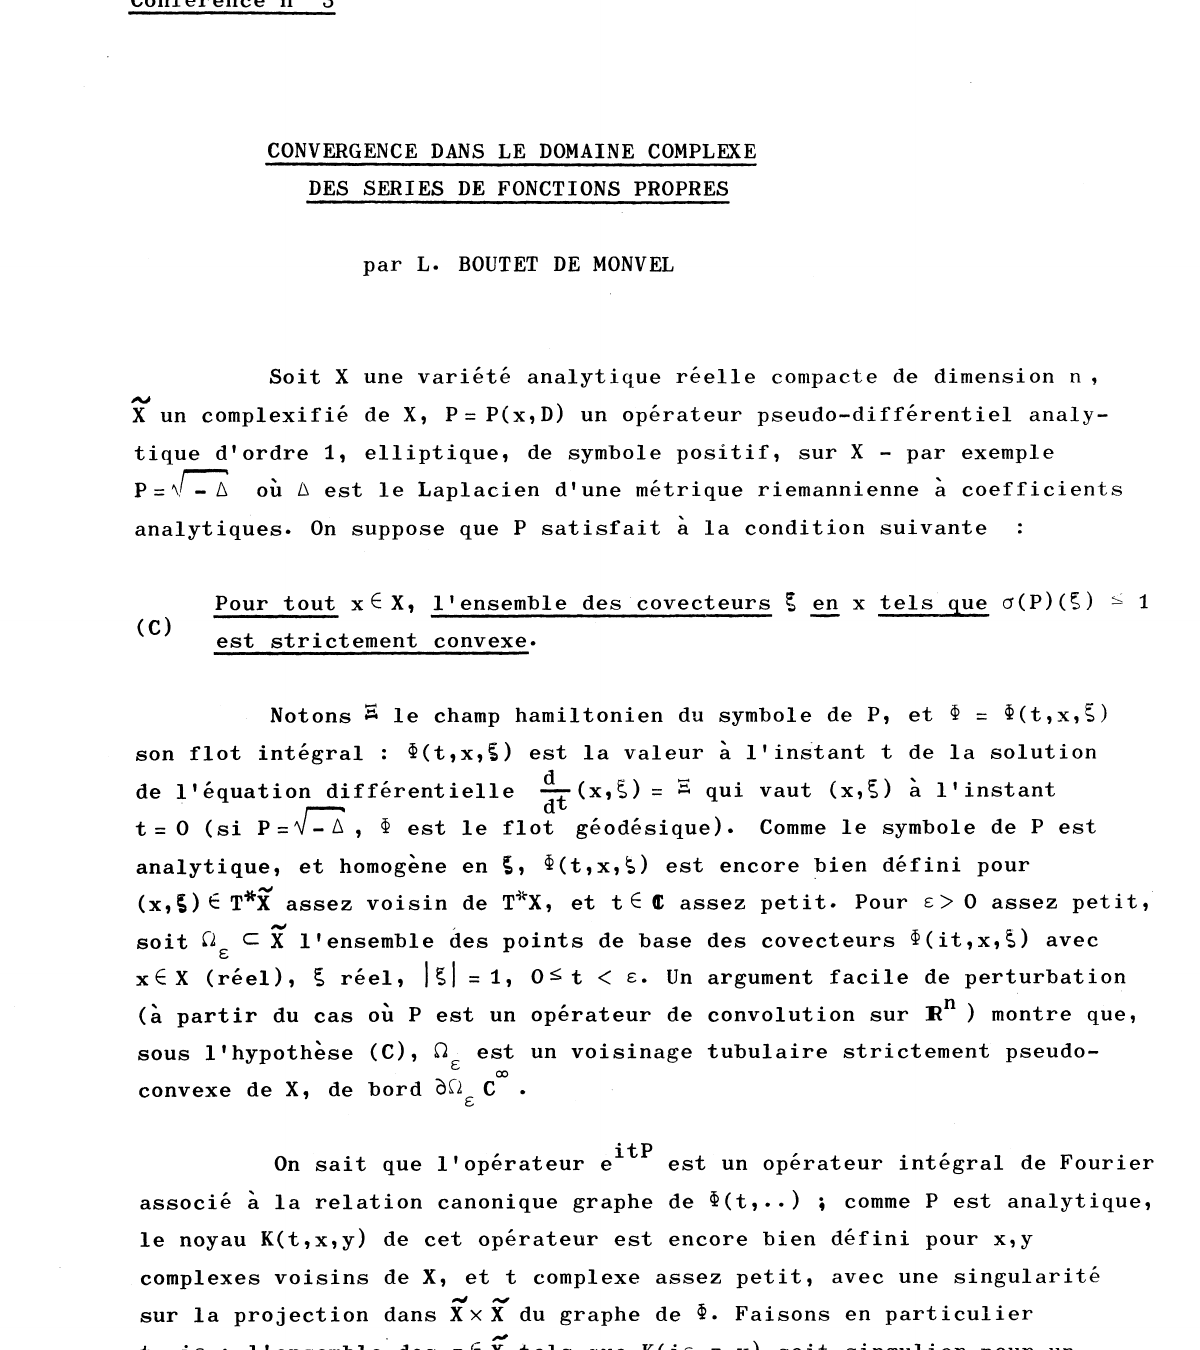
\includegraphics[width=0.95\linewidth]{figures/original_boutet_condition_crop.png}
  \caption{Boutet de Monvel's set-theoretic condition (C), followed by the
  asserted smooth strictly pseudoconvex tube conclusion.}
  \label{fig:original}
\end{figure}

\section{Proof intuition}

For a translation-invariant principal root $q=p^{1/d}$, put
$F=q^2/2$.  The conjectured positive imaginary-time flow is simply
\[
 \Phi(x,\xi)=x+i\nabla F(\xi).
\]
Its Jacobian contains $D^2F$, so segment-strictness without positive curvature
cannot give the claimed diffeomorphism.  This produces the $\ell^4$
counterexample.

There is a separate sign obstruction.  If $q$ is not reversible, the Legendre
image of the positive imaginary flow is
\[
 D_\eps^+=\{v:q^*(v)<\eps\},
\]
whereas the Fourier factor
$\ee^{-\eps q(k)}\ee^{ik(x+iv)}$ decays precisely on
\[
 D_\eps^- =\{v:q^*(-v)<\eps\}=-D_\eps^+.
\]
The two tubes agree exactly when $q(\xi)=q(-\xi)$.  A Randers gauge
$q(\xi)=|\xi|+c\xi_1$ has an ellipsoidal, everywhere positively curved unit
ball but is not reversible, so the kernel grows exponentially at points of
the conjectured tube.  This defeats the strong-curvature interpretation as
well.

The same two observations are also sufficient.  Positive $D^2F$ gives the
Legendre diffeomorphism and a nondegenerate complex phase; reversibility makes
the flow tube equal the Fourier holomorphy tube.  A lower-order classical term
only multiplies the boundary FIO by an elliptic order-zero amplitude.  This
yields the exact flat-torus characterization below.

\section{A positive-curvature counterexample}

Let $n\geq2$, $0<c<1$, and use $D_j=-i\partial_{x_j}$ on the flat analytic
torus $\T^n$.  Define
\begin{equation}\label{eq:randersP}
 P=(-\Delta)^{1/2}+cD_1,
 \qquad
 q(\xi)=|\xi|+c\xi_1.
\end{equation}

\begin{theorem}[Counterexample independent of convexity terminology]
\label{thm:randers}
The operator \eqref{eq:randersP} satisfies every hypothesis printed before
Winterrose's Conjecture~4.1.  Its unit principal co-ball is an ellipsoid and
has everywhere positive-definite second fundamental form; equivalently,
$D^2(q^2/2)$ is positive definite off the zero section.  Nevertheless, for
every $\eps>0$, the kernel of $\ee^{-\eps P}$ does not extend holomorphically
to the tube $M_\eps^\Phi$ prescribed by conclusion~\textnormal{(1)}.  Thus
conclusion~\textnormal{(4)}, and hence the full conjecture, is false even under
the strong-curvature interpretation of ``strictly convex.''
\end{theorem}

\begin{proof}
On the Fourier basis $e_k(x)=e^{ik\cdot x}$,
\[
 Pe_k=q(k)e_k=(|k|+ck_1)e_k.
\]
Hence $P$ is an analytic classical polyhomogeneous pseudodifferential operator
of order $d=1$, formally self-adjoint and nonnegative.  Its principal symbol
is positive and elliptic because
\[
 (1-c)|\xi|\leq q(\xi)\leq(1+c)|\xi|.
\]
It has no negative eigenvalues.  Its symbol is independent of $x$, so its
real Hamilton flow is complete and entire in time.

The unit co-ball is much stronger than segment-strict.  Squaring
$|\xi|\leq1-c\xi_1$ gives
\begin{equation}\label{eq:ellipsoid}
 (1-c^2)\left(\xi_1+\frac{c}{1-c^2}\right)^2
 +|\xi'|^2\leq\frac1{1-c^2}.
\end{equation}
Conversely every point of this ellipsoid has $1-c\xi_1>0$, so
\eqref{eq:ellipsoid} is exactly $\{q\leq1\}$.  It is a smooth ellipsoid with
positive curvature everywhere.

For completeness, put $r=|\xi|$ and $u=\xi/r$.  For any $\eta\neq0$,
\begin{align*}
 D^2\left(\frac{q^2}{2}\right)(\xi)[\eta,\eta]
 &=(u\cdot\eta+c\eta_1)^2
 +(1+cu_1)\bigl(|\eta|^2-(u\cdot\eta)^2\bigr)>0.
\end{align*}
Indeed the second summand is positive unless $\eta$ is parallel to $u$, and
in the parallel case the first is positive because $1+cu_1\geq1-c>0$.

Let $F=q^2/2$.  The Hamilton flow of $q$ is
$\varphi_t(x,\xi)=(x+t\nabla q(\xi),\xi)$, and therefore the map prescribed in
the conjecture is
\begin{equation}\label{eq:randersPhi}
 \Phi(x,\xi)=x+i q(\xi)\nabla q(\xi)=x+i\nabla F(\xi).
\end{equation}
Positive definiteness just proved makes it a real-analytic Legendre
diffeomorphism.  In particular, along the positive first axis,
\[
 \nabla F(te_1)=(1+c)^2t e_1,
 \qquad q(te_1)=(1+c)t.
\]
Taking $t=\eps/(1+c)^2$ shows that
\begin{equation}\label{eq:vinside}
 z=x+i\eps e_1\in M_\eps^\Phi;
\end{equation}
the inequality $q(te_1)=\eps/(1+c)<\eps$ is strict.

The Schwartz kernel on the real torus is
\begin{equation}\label{eq:randerskernel}
 K_\eps(x,y)=(2\pi)^{-n}\sum_{k\in\Z^n}
 e^{-\eps q(k)}e^{ik\cdot(x-y)}.
\end{equation}
Suppose it extended holomorphically to the point \eqref{eq:vinside} for a
fixed $y$.  Restricting the extension to the real $x$-torus at height
$v=\eps e_1$, uniqueness of analytic continuation forces its $k$th Fourier
coefficient to be
\[
 e^{-\eps q(k)}e^{-k\cdot v}e^{-ik\cdot y}.
\]
For $k=-me_1$, $m\to\infty$, its modulus is
\[
 e^{-\eps m(1-c)}e^{\eps m}=e^{c\eps m}.
\]
These coefficients grow exponentially.  They cannot be the Fourier
coefficients even of a distribution, much less of a real-analytic function.
This contradiction proves failure of conclusion~(4).
\end{proof}

\begin{remark}[Scope of the new obstruction]
Boutet de Monvel's original note is formulated for scalar differential
operators.  Positivity forces their order to be even, and their homogeneous
principal polynomial is then even in $\xi$.  Thus reversibility is automatic
in that original scope.  Winterrose explicitly changes the statement to
general $P\in\Psi^d_{\mathrm{phg}}(M)$, where formal self-adjointness only
makes the principal symbol real, not even.  Theorem~\ref{thm:randers} refutes
that published pseudodifferential formulation.  If ``the intended theorem''
also silently retains the original differential-operator scope, then the
example instead identifies a second missing hypothesis in the generalization.
\end{remark}

\section{The segment-strict curvature counterexample}

The earlier ambiguity is real and yields a separate obstruction.  On $\T^2$
take
\begin{equation}\label{eq:l4P}
 P=\partial_1^4+\partial_2^4,
 \qquad p(\xi)=\xi_1^4+\xi_2^4,
 \qquad q=p^{1/4}.
\end{equation}
This is a nonnegative, formally self-adjoint analytic elliptic differential
operator.  Its $\ell^4$ unit co-ball has no boundary segments because
$t\mapsto|t|^4$ is strictly convex.

\begin{proposition}[Failure under the literal convex-set convention]
For \eqref{eq:l4P}, the flow map in conclusion~\textnormal{(1)} is not a local
diffeomorphism at any nonzero axial covector, for any radius.  Its image
boundary is only $C^1$ at the corresponding axes, so conclusion~\textnormal{(2)}
also fails.
\end{proposition}

\begin{proof}
Here
\[
 F(\xi)=\frac12q(\xi)^2
 =\frac12(\xi_1^4+\xi_2^4)^{1/2},
 \qquad \Phi(x,\xi)=x+i\nabla F(\xi).
\]
At $(a,0)$, $a\neq0$,
\[
 D^2F(a,0)=\begin{pmatrix}1&0\\0&0\end{pmatrix},
 \qquad
 D\Phi=\operatorname{diag}(I_2,D^2F),
\]
so $D\Phi$ has rank three.  Shrinking the tube cannot remove this defect.

The image is the dual-gauge tube with
\[
 q^*(v)=\bigl(|v_1|^{4/3}+|v_2|^{4/3}\bigr)^{3/4}.
\]
Near $(\eps,0)$ its boundary is
\[
 v_1=(\eps^{4/3}-|v_2|^{4/3})^{3/4}
 =\eps-\frac34\eps^{-1/3}|v_2|^{4/3}
 +O(|v_2|^{8/3}).
\]
The second derivative is unbounded at zero, so the boundary is not $C^2$ and
cannot be real analytic.
\end{proof}

\section{Complete translation-invariant characterization}
\label{sec:characterization}

The two examples give all the obstructions in the flat constant-coefficient
class, including classical lower-order terms.  Let
$q:\R^n\to[0,\infty)$ be positive, one-homogeneous and real analytic away
from zero, with strictly convex unit co-ball.  It need not be even.  Let
$\mu$ be a positive real-analytic classical symbol of order one with principal
part $q$, so
\begin{equation}\label{eq:muclassical}
 \mu(\xi)=q(\xi)+r(\xi),\qquad r\in S^0_{\mathrm{cl}}.
\end{equation}
Changing finitely many lattice values is harmless.  For $d>0$, define
\begin{equation}\label{eq:classicalmult}
 Pe_k=\mu(k)^d e_k.
\end{equation}
Then $P$ is a nonnegative, self-adjoint, translation-invariant classical
operator of order $d$, with principal symbol $p=q^d$ and
$P^{1/d}e_k=\mu(k)e_k$.

Write $F=q^2/2$ and let
\[
 q^*(v)=\sup_{q(\xi)=1}v\cdot\xi
\]
be the polar gauge.  Reversibility means $q(-\xi)=q(\xi)$.

\begin{theorem}[Exact flat-torus repair]
\label{thm:characterization}
For the class \eqref{eq:classicalmult}, the following are equivalent:
\begin{enumerate}[label=\textnormal{(\roman*)}]
\item all six conclusions of Winterrose's Conjecture~4.1, with its printed
      positive imaginary-time map, hold for some (equivalently every)
      $\eps>0$;
\item $D^2F(\xi)$ is positive definite for every $\xi\neq0$ and $q$ is
      reversible.
\end{enumerate}
If only $D^2F>0$ is assumed, the kernel is holomorphic on the reflected tube
\[
 \T^n+i\{v:q^*(-v)<\eps\},
\]
and all six conclusions hold after replacing the positive imaginary-time map
by the negative one, $\Phi_-(x,\xi)=x-i\nabla F(\xi)$.
\end{theorem}

\begin{proof}
For every $q$ in the class, the positive imaginary-time flow is
\begin{equation}\label{eq:generalPhi}
 \Phi_+(x,\xi)=x+i\nabla F(\xi),
 \qquad D\Phi_+=\operatorname{diag}(I_n,D^2F(\xi)).
\end{equation}
Since the unit co-ball is convex, $F$ is convex and $D^2F$ is positive
semidefinite.  Conclusion~(1) therefore forces it to be positive definite.

Assume this positivity for the moment.  Fenchel duality gives
\[
 F^*(v)=\frac12q^*(v)^2,
 \qquad
 \nabla F:\R^n\setminus0\longrightarrow\R^n\setminus0
\]
as a real-analytic diffeomorphism with inverse $\nabla F^*$, and
$q^*(\nabla F(\xi))=q(\xi)$.  Hence the tube in conclusion~(1) is
\begin{equation}\label{eq:positiveTube}
 M_\eps^{\Phi_+}=\T^n+iD_\eps^+,
 \qquad D_\eps^+=\{v:q^*(v)<\eps\}.
\end{equation}

The kernel is
\begin{equation}\label{eq:generalkernel}
 K_\eps(z,y)=(2\pi)^{-n}\sum_{k\in\Z^n}
 e^{-\eps\mu(k)}e^{ik\cdot(z-y)}.
\end{equation}
Because $\mu(k)=q(k)+O(1)$, its maximal open tube of normal Fourier
convergence is
\begin{equation}\label{eq:negativeTube}
 D_\eps^-=\{v:q^*(-v)<\eps\}=-D_\eps^+.
\end{equation}
More explicitly, if $q^*(-v)>\eps$, lattice directions approximate a support
direction for $-v$, and the corresponding coefficients in
\eqref{eq:generalkernel} grow exponentially.  They are not Fourier
coefficients of a distribution.  Thus conclusion~(4) on all of
$D_\eps^+$ implies
\[
 q^*(-v)\leq q^*(v)\quad(v\in\R^n).
\]
Applying this to $-v$ gives equality.  Hence $q^*$, and therefore $q$, is
even.  This proves necessity of both conditions.

Conversely, assume $D^2F>0$ and reversibility.  Then
$D_\eps^+=D_\eps^-$, so \eqref{eq:generalPhi} and Legendre duality prove
conclusion~(1).  A real-analytic defining function near the boundary is
\[
 \rho(x+iv)=2F^*(v)-\eps^2.
\]
Its complex Levi form is a positive multiple of $D^2F^*(v)$, proving the
real-analytic boundary and strict pseudoconvexity in conclusions~(2)--(3).
Duality gives normal convergence of \eqref{eq:generalkernel}, with all
derivatives, on compact subsets of the tube, proving conclusion~(4).

On $q^*(v)=\eps$, write
\[
 e^{-\eps\mu(\xi)}
 =e^{-\eps q(\xi)}b_\eps(\xi),
 \qquad b_\eps=e^{-\eps(\mu-q)}\in S^0_{\mathrm{cl}}.
\]
The amplitude $b_\eps$ is elliptic.  Poisson summation gives, modulo a smooth
kernel, the positive complex phase
\[
 \phi(x,v,y,\xi)
 =(x-y)\cdot\xi+i\bigl(\eps q(\xi)+v\cdot\xi\bigr).
\]
Its imaginary part is nonnegative and vanishes exactly at
$x=y$ and $v=-\eps\nabla q(\xi)$.  Positive $D^2F$ makes the canonical graph
nondegenerate.  With $n$ phase variables, target dimension $2n-1$, source
dimension $n$, and order-zero amplitude, the standard order formula gives
\[
 \frac n2-\frac{(2n-1)+n}{4}=-\frac{n-1}{4}.
\]
This proves conclusion~(5) by the positive complex-phase calculus
\cite{Hormander,MelinSjostrand}.

Finally, for any smooth positive boundary density, the $k$th eigenvalue of
$S_\eps^*S_\eps$ is
\[
 e^{-2\eps\mu(k)}
 \int_{q^*(v)=\eps}e^{-2k\cdot v}a(v)\,d\sigma(v).
\]
Laplace's method at the unique nondegenerate support point
$v=-\eps\nabla q(k)$ makes this an elliptic classical symbol of order
$-(n-1)/2$; the order-zero factor from $\mu-q$ does not change the order.
Thus
\[
 \|S_\eps f\|_{H^{s+(n-1)/4}}
 \asymp \|f\|_{H^s}.
\]
The range is closed and contains every holomorphic Fourier polynomial, since
all Fourier multipliers are nonzero.  Such polynomials are dense in the
source paper's definition of
$\cO^{s+(n-1)/4}(\partial M_\eps^{\Phi_+})$, so the range is the entire space.
This is conclusion~(6).

If reversibility is dropped, repeat the same argument on
$D_\eps^-=-D_\eps^+$ with
$\Phi_-(x,\xi)=x-i\nabla F(\xi)$.  The phase and its critical support point
are then aligned exactly as above, proving the sign-corrected statement.
\end{proof}

\section{What this says about the intended theorem}

There are now three distinct readings, and the result is useful in each.
\begin{enumerate}
\item Under the literal no-segments definition, the $\ell^4$ differential
      operator directly refutes conclusions~(1)--(2).
\item If ``strictly convex'' means positive curvature, the $\ell^4$ example is
      excluded, but the Randers multiplier still refutes Winterrose's printed
      pseudodifferential formulation through conclusion~(4).
\item If the intended statement silently combines positive curvature with
      Boutet de Monvel's original differential-operator scope, both
      obstructions have been excluded by intent.  In that case this packet is
      a precise statement correction rather than a refutation of the intended
      theorem.  Theorem~\ref{thm:characterization} remains a complete result:
      it proves all six conclusions for every strongly convex reversible
      classical multiplier, including arbitrary classical lower-order terms,
      and identifies the exact additional repair needed for nonreversible
      pseudodifferential symbols.
\end{enumerate}

The variable-coefficient, strongly convex, reversible case on a general
analytic manifold remains open.  The geometric part should be locally stable
under small radius because the leading Legendre Hessian is nondegenerate, but
conclusions~(4)--(6) require the global analytic half-wave/FIO construction
that Winterrose's thesis itself identifies as the unresolved core.  No claim
to solve that general problem is made here.

\section{Verification and novelty notes}

\begin{enumerate}
\item \textbf{Hypotheses and failures.}  Every printed condition was checked
      for the Randers operator, including strong convexity and the flow
      assumptions; its failure is exponential Fourier growth.  The $\ell^4$
      failure is independently a rank defect and a non-$C^2$ boundary.
\item \textbf{Version audit.}  ArXiv v1--v3, the published text, the original
      note, and thesis Sections~7.1--7.2 contain neither a convexity definition
      nor an evenness hypothesis.
\item \textbf{Bounded novelty search.}  On 22 July 2026 the run indexes and
      web/arXiv were searched by the source id/title and combinations of
      strict/strong convexity, $\ell^4$, Randers, nonreversibility,
      $|\xi|+c\xi_1$, and imaginary Hamilton flow.  No prior counterexample or
      this characterization was found; this is not exhaustive certification.
\end{enumerate}

\paragraph{Human-review recommendation.}
Prioritize Theorem~\ref{thm:randers}: check the source's flow sign and its
standard inclusion of the analytic classical multiplier $|D|+cD_1$.  Then
review the complex-phase and Laplace steps in
Theorem~\ref{thm:characterization}.  Author clarification can still decide
whether the intended scope retained both strong curvature and differential
operators.

\begin{thebibliography}{9}
\small
\setlength{\itemsep}{0pt}

\bibitem{Winterrose}
D. S. Winterrose,
\emph{Algebras of pseudo-differential operators acting on holomorphic Sobolev
spaces}, J. Funct. Anal. \textbf{285} (2023), article 109972;
arXiv:2110.09389v3.

\bibitem{Boutet1979}
L. Boutet de Monvel,
\emph{Convergence dans le domaine complexe des s\'eries de fonctions propres},
Journ\'ees \'Equations aux d\'eriv\'ees partielles (1979), article no.~3,
1--2, DOI: 10.5802/jedp.189.

\bibitem{WinterroseThesis}
D. S. Winterrose,
\emph{Complexifications, Pseudo-Differential Operators, and the Poisson
Transform}, Ph.D. thesis, Technical University of Denmark, 2021.

\bibitem{Hormander}
L. H\"ormander,
\emph{Fourier integral operators. I}, Acta Math. \textbf{127} (1971), 79--183.

\bibitem{MelinSjostrand}
A. Melin and J. Sj\"ostrand,
\emph{Fourier integral operators with complex-valued phase functions},
Lecture Notes in Math. \textbf{459}, Springer (1975), 120--223.

\end{thebibliography}

\end{document}
